\documentclass[12pt]{article}
\usepackage{geometry}
\usepackage{dcolumn}
\usepackage{booktabs}
\usepackage{pdflscape}
\usepackage{graphicx}
\usepackage{placeins}
\usepackage{dcolumn}
\usepackage{booktabs}
\linespread{1.5}
\usepackage{subcaption}
\usepackage{amsmath}
\usepackage{hyperref}
\usepackage{xepersian}
\settextfont{XB Zar}
\setdigitfont{XB Zar}

\begin{document}
\title{سهام‌های مرتبط}
\author{سید مرتضی آقاجان‌زاده}
\maketitle

با توجه به سهام دار مشترک میان دو نماد موجود در بازار، سهام‌های مرتبط تعریف می‌شوند. با کنترل ویژگی‌های دو نماد و شباهت‌های میان بخشی آیا با افزایش درجه‌ی سهامداری مشتترک، رفتار قیمتی دو نماد تغیر می‌کند؟ 

عدم تقارن اطلاعاتی و دسترسی بیشتر به اطلاعات شركت توسط سهامدار كنترلی
باعث می شود كه سهامدار عمده در زمان رونق كسب و كار با ممانعت از افشای اطلاعات، سود بیشتر از حق خود را كسب
كند. در مقابل، زمانی كه كسب و كار دچار ضرر یا ركود شود، سهامدار كنترلی با انتشار اطلاعات می تواند دیگران را در این
زیان شریك كند.

عدم افشای اطلاعات مخصوص شركت و در نتیجه عدم انعكاس آن در قیمت سهام به این معناست كه بخش
بزرگ تری از اطلاعات انعكاس یافته در قیمت و در نتیجه نوسان های بازده، از اطلاعات سیستماتیك نشئت م یگیرد كه
این باعث می شود حركت هم جهت قیمت ها یا به اصطلاح هم زمانی  بازده افزایش یابد. این سازوكار بر عدم شفافیت
اطلاعات شركت ها و در نتیجه عدم انعكاس اطلاعات مخصوص شركت در قیمت سهام مبتنی است.
\section{مطالعات گذشته}
\subsection{\lr{Connected Stocks}}
این مقاله به بررسی رفتار سهام‌های یکسان در سبد سرمایه‌گذاری صندوق‌های سرمایه‌گذاری مشترک می‌پردازد. در این مقاله جهت بررسی درجه اشتراک مالکیت میان دو نماد از  تقسیم تمام ارزش مالکیت مشترک میان دو نماد بر کل ارزش بازاری دو نماد استفاده می‌شود و در ادامه با نماد $ FCAP_{ij,t} $ نشان داده می‌شود. به عبارت دیگر این متغیر برابر است با:
\begin{equation}
 FCAP_{ij,t} = \frac{\sum_{f = 1}^{F} (S^f_{i,t}P_{i,t}+S^f_{j,t}P_{j,t})}{S_{i,t}P{i,t} + S_{j,t}P{j,t}} 
 \label{e2}
\end{equation}
 که 
 $ S^f_{i,t} $
 بیانگر مالیکت سهام i در زمان t توسط صندوق f و
  $ P_{i,t}$
  قیمت همان سهام در زمان t می‌باشد. 
  منظور از مالکیت مشترک در لحظه t، وجود سهام‌دار عمده مشترک برای دو نماد i و j در این لحظه می‌باشد. به دلیل قابل مقایسه بودن این ملاک میان جفت نماد‌های متفاوت در هر جفت، این پارامتر ابتدا تبدیل رتبه‌ای
  \LTRfootnote{rank-transformed}
   شده‌است و پس از آن نرمال شده است و پارامتر نرمال شده با $ FCAPF^*_{ij,t} $ نشان داده شده‌است.(میانگین به صفر و انحراف معیار به یک تغییر یافته است) 
  
  در این مقاله هم بستگی باقی مانده 
  \LTRfootnote{\lr{Residuals}}
  پیش بینی بازده ماهانه به وسیله مدل چهار عاملی میان دو سهام را مورد بررسی قرار می‌دهد. مدل مورد بررسی مقاله در رابطه 
  \ref{e1}
  بیان شده است. در این مدل پارامتر مورد بررسی $ b_f $ می‌باشد.
  
  \begin{equation}
  \rho_{ij,t+1} = a + b_f \times FCAPF^*_{ij,t} + \sum_{k = 1}^{n } CONTROL_{ij,t,k} + \varepsilon_{ij,t+1}
  \label{e1}
  \end{equation}
  مقاله از کنترل‌های متنوعی استفاده می‌کند. دغدغه اصلی نگارنده  وجود درون‌زایی‌های ناشی از ملاک‌های انتخاب توسط مدیران صندوق‌های می‌باشد. در شکل 
  \ref{g1}
   خروجی‌های مدل مقاله ارائه شده‌است. متغیر 
   $ A_{ij,t} $
  تعداد تحلیلگران بازار مالی است که برای دو سهم i و j حداقل یک گزارش مالی سالانه منتشر کرده باشند. 
  برای کنترل شباهت‌ دو سهام، یکی از مشخصات شباهت را در هر دوره براساس صدک رتبه‌بندی می‌کنیم و پارامتر مورد بررسی از منفی مقدار اختلاف تفاوت صدکی این ملاک شباهت می‌باشد. در مقاله از مشخصات اندازه، B/M و نوسان سهم استفاده شده‌است.
  \begin{figure}[htbp]
  \centering
  \includegraphics[width=\columnwidth]{Table1.png}
  \caption{ خروجی مدل مقاله \lr{Connected Stocks} }
  \label{g1}
 
  \end{figure}  
\FloatBarrier


\subsection{ساختار بنگاه داری و رفتار بازده سهام: شواهدی از بورس اوراق بهادار تهران}
\label{s1.2}
در این پژوهش ابتدا این سؤال بررسی می شود كه ابعاد و ساختار بنگاه داری هرمی و ضربدری در ایران چگونه و
به چه میزان است؟ در این راستا از سه تعریف شبكه های مدیریتی، سهامداری و مالكیتی بهره گرفته شده است؛ در
شبكه مدیریتی، در صورت وجود عضو مشترك بین مدیران ارشد شامل اعضای هیئت مدیره و مدیرعامل دو شركت، آن
دو را مرتبط در نظر گرفته‌است. در شبكه سهامداری، چنانچه شركتی سهامدار شركت دیگر باشد و  در شبكه مالكیتی به واسطه وجود یك سهامدار مشترك دو شركت را مرتبط در نظر گرفته‌است. در شکل‌های 
\ref{m}-\ref{h}
گراف شبکه‌های متفاوت رسم شده‌است.

\begin{figure}[htbp]
\centering
  \includegraphics[width=0.6\linewidth]{m.png}
  \caption{گراف شبکه مدیریتی }
  \label{m}
 \end{figure} 
\begin{figure}[htbp]
\centering
  \includegraphics[width=0.6\linewidth]{h1.png}
  \caption{گراف شبکه سهامداری برای آستانه 30 درصد }
  \label{h1}
 \end{figure}
 \begin{figure}[htbp]
 \centering
   \includegraphics[width=0.6\linewidth]{h.png}
   \caption{گراف شبکه مالکیت برای آستانه 30 درصد }
   \label{h}
  \end{figure}
%\newpage
\FloatBarrier

در ادامه برای مقایسه هم بستگی بازده‌های سهم‌های موجود در شبکه‌های تعریف شده از بازده هفتگی سهم استفاده شده‌است و جهت از بین بردن عوامل برونزا از بازده روند زدایی شده استفاده کرده است که در روایط زیر تعریف شده‌است.
\begin{equation}
r_{i,t} = \alpha_i +\beta_i t + \varepsilon_{i,t} \rightarrow r_{i,t} = \hat{\alpha}_i +\hat{\beta}_i t + r^d_{i,t} \Rightarrow r^d_{i,t} = r_{i,t} -\hat{\alpha}_i -\hat{\beta}_i t 
\end{equation}
پس تعریف بازده روندزدایی شده به منظور مقایسه همبستگی دو سهم از دو متغیر وابسته متفاوت تعریف می‌کند. متغیر $ f_{i,j} $ که است از هم حرکتی دو سهم در هفته‌های متفاوت می‌باشد. در این رابطه، $ n_{i,j,t}^{up} $ اگر در هفته $ t $، بازده دو شرکت i و j مثبت باشد برابر با 1 و در غیر این صورت صفر است. به صورت مشابه $ n_{i,j,t}^{down} $ برای بازده منفی تغریف شده‌است. $ T_{i,j} $ تعداد کل هفته‌های مورد بررسی می‌باشد.اگر شاخص هم حركتی را با بازده های روندزدایی شده محاسبه كنیم ، آن را شاخص هم حركتی
 روندزدایی شده می‌نامد و به صورت $ f^d_{i,j} $ نشان می‌دهد.
\begin{equation}
f_{i,j}  = \frac{\sum_t (n_{i,j,t}^{up}+n_{i,j,t}^{down})}{T_{i,j}}
\end{equation}
متغیر وابسته دیگری که تعریف می‌کند هم بستگی بازده دو سهم می‌باشد که با $ C_{i,j} $ نشان می‌دهد. در تعریف این پارامتر نیز چنانچه از بازده روندزدایی شده استفاده کرده باشد به آن هم بستگی روندزدایی شده می‌گوید و با $ C^d_{i,j} $ نشان می‌دهد.

با توجه به تعریف متغیر‌های وابسته، متغیر هم حركتی روندزدایی شده و روندزدایی نشده، هر دو در بازه $ [0,1] $ قرار دارد و متغیر همبستگی روندزدایی شده و روندزدایی نشده نیز در بازه $ [-1,1] $ قرار دارد. با توجه به اینکه مشاهدات نقاط مرزی این پژوهش قابل توجه نبوده‌است از تبدیل لجستیک برای این متغیر‌ها استفاده کرده‌است. نتایج رگرسیون حداقل مربعات در شکل‌های 
\ref{g2} 
و
\ref{g3}
نشان داده شده‌است.
\begin{equation}
\psi_{i,j}^d = \log(\frac{C^d_{i,j}+1}{1-C^d_{i,j}})
\end{equation}

\begin{equation}
\phi_{i,j}^d = \log(\frac{f^d_{i,j}}{1-f^d_{i,j}})
\end{equation}



\begin{landscape}
\begin{figure}
\centering
\includegraphics[width=\columnwidth]{Table2.png}
\caption{نتایج رگرسیون حداقل مربعات برای عضویت شرکت‌ها در شبکه‌های مختلف و ارتباط دو به دویی}
\label{g2}
\end{figure}
\begin{figure}
\centering
\includegraphics[width=\columnwidth]{Table3.png}
\caption{نتایج رگرسیون حداقل مربعات برای عضویت شرکت‌ها در شبکه‌های مختلف و فاصله آن‌ها در هر شبکه}
\label{g3}
\end{figure}
\end{landscape}

\section{نتایج مقاله با داده‌های ایران}
در داده‌های ایران ارتباط نماد‌های مختلف براساس سهامدار مشترک مورد بررسی قرار گرفته‌است. با توجه به رابطه 
\ref{e2}
پارامتر 
$ FCAPf $ 
را تعریف کردیم و با توجه به مقاله بر روی آن تبدیل رتبه‌ای نرمال شده انجام دادیم. از طرفی دیگر برای از بین بردن همسانی ساختاری دو بنگاه از هم بستگی باقی‌مانده‌های برآورد مدل چهار عاملی به صورت هفتگی استفاده شده‌است. نتایج  رابطه همبستگی با متغیر تعریف شده برای مالکیت مشترک برای تبدیل نیافته و تبدیل یافته در شکل 
\ref{f1} 
و 
\ref{f2}
نشان داده شده‌است.
 




\lr{\begin{LTR}
\begin{figure}[htbp]
  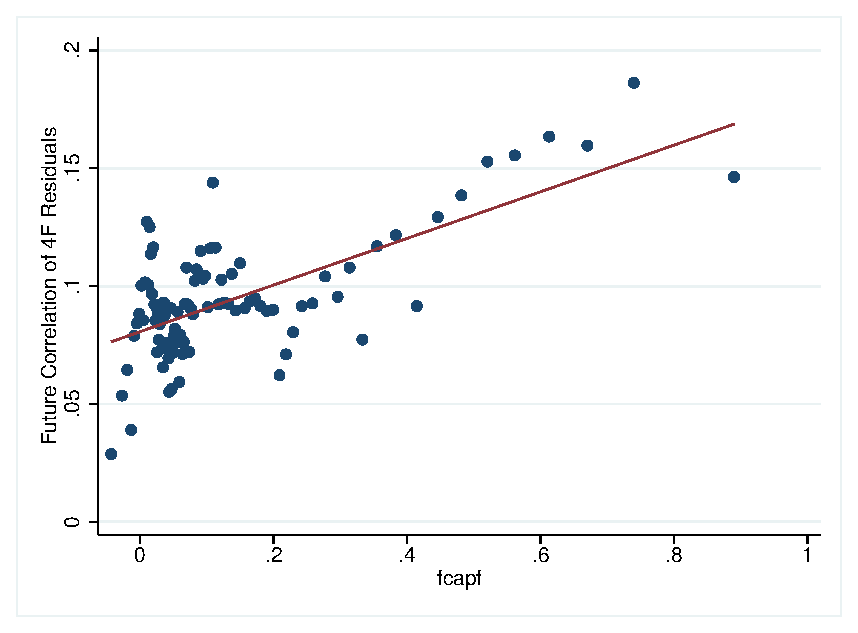
\includegraphics[width=.5\linewidth]{mygraph2.eps}\hfill
  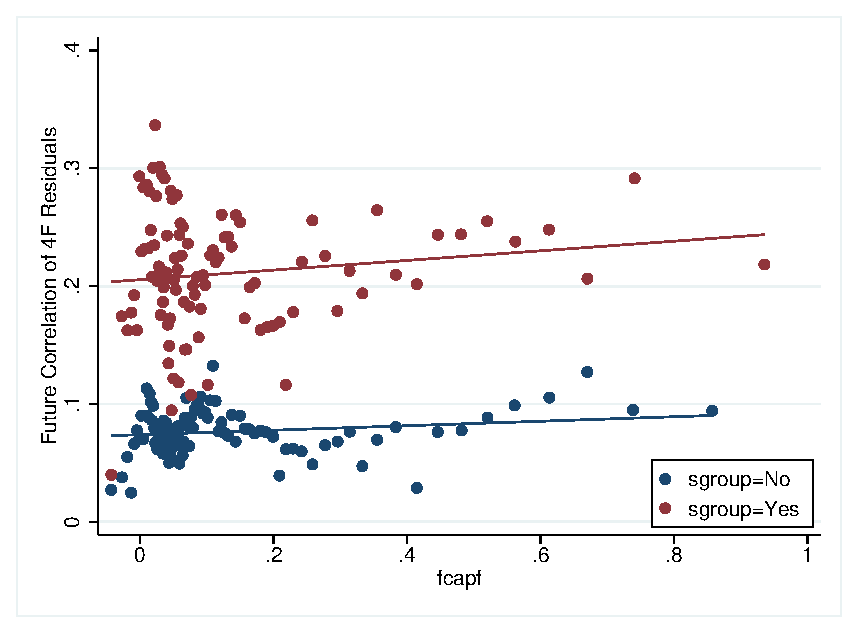
\includegraphics[width=.5\linewidth]{mygraph.eps}
  \caption{{Correlation of 4F Residuals via fcapf}}
  \label{f1}
 \end{figure} 
 \end{LTR}}
 \lr{\begin{LTR} 
\begin{figure} [htbp]
    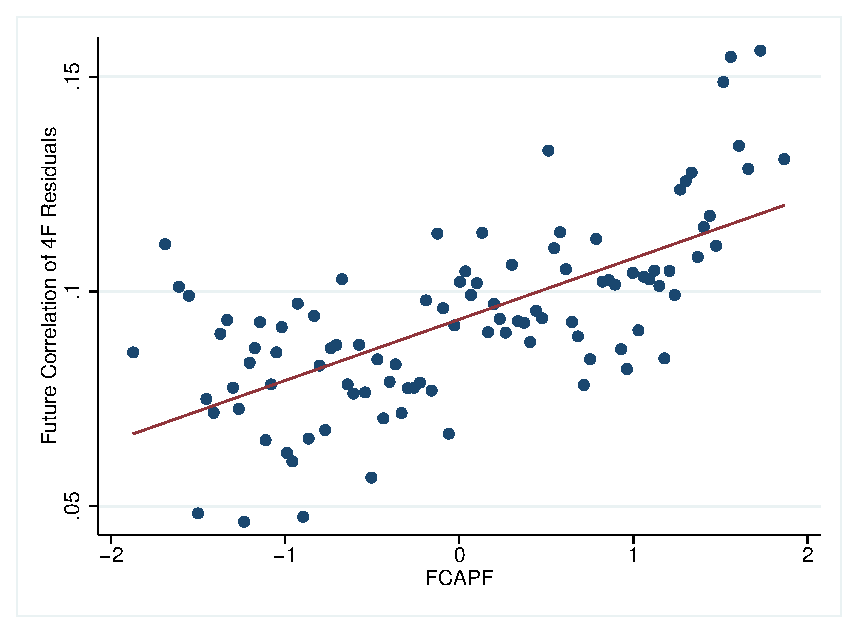
\includegraphics[width=.5\linewidth]{mygraph4.eps}\hfill
    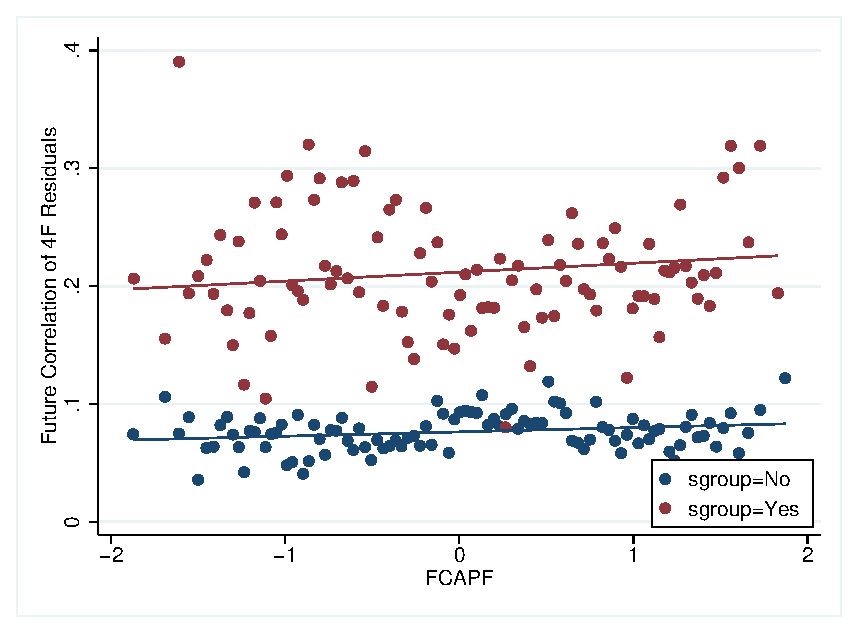
\includegraphics[width=.5\linewidth]{mygraph3.eps}
    \caption{{Correlation of 4F Residuals via $ \text{FCAPF}_{\text{(Normalized Rank-Transformed of  fcapf)}} $}}
    \label{f2}
\end{figure}
\end{LTR}}
\FloatBarrier
علاوه بر از بین بردن روند‌های موجود در بازده سهام به وسیله مدل چهارعاملی از کنترل‌های دیگر نیز استفاده شده است.  برای تفکیک اثر یکسانی رفتار دو سهم، 
$ \text{sgroup} $
می‌باشد تا چنانچه دو سهم به یک گروه صنعتی تعلق داشته باشند آنگاه مقدار آن برابر یک خواهد شد. دیگر کنترل جهت یکسانی اندازه دو سهم 
$ \text{samesize} $
است که برابر منفی اختلاف رتبه صدکی اندازه دو سهم می‌باشد. متغیر 
$ \text{size} $ 
نیز همین رتبه صدکی اندازه سهم می‌باشد که در کلیه جداول منظور از 
شرکت 1 شرکت بزرگتر است. یکی دیگر از کنترل‌های مورد استفاده هم بستگی در دوره‌ی $ t $ می‌باشد.

در جدول
\ref{t1} 
و
\ref{t4}
خلاصه نتایج برآورد برای مدل‌های متفاوت به ازای متغیر‌های کنترل بیان شده‌است و به ترتیب شامل نتایج  برآورد‌ها براساس محاسبات ساده 
$ \text{fcapf} $
 و
 $ \text{FCAPF} $ 
 می‌باشد. 
 با توجه به مشخصات سهام و حذف اثر اندازه به وسیله مدل چهار عاملی به نظر می‌آید استفاده از مدل شماره 5 به منظور برآورد مدل از توضیح دهندگی بالاتری برخوردار باشد. به همین جهت پیش‌بینی‌های مدل 5 برای دو عامل در جدول
 \ref{t2} 
 به ازای متغیر وابسته در دوره
  $ t+1 $
  و
  $ t+2 $
  بیان شده‌است.
  در جدول 
  \ref{t3}
  نتایج با روش اثر ثابت در سطح شرکت‌های مشترک آورده شده‌است. در این سری محاسبات به دلیل عدم تغییر قابل توجه متغیر 
  $ samesize $
  از اندازه خود شرکت‌ها و حاصل ضرب آن‌ها استفاده شده‌است. سپس با توجه به قرار گرفتن متغیر‌های هم بستگی در بازه $  [-1,1] $ و متغیر $ fcapf $ در بازه $ [0,1] $  از تبدیل لجستیک استفاده شده در مقاله 
  \ref{s1.2}
   کردیم. هیستوگرام متغیر‌های تبدیل شده در شکل 
   \ref{g4}
   نشان داده شده‌است. نتایج معادلات با توجه به این تبدیل  و شیوه‌های مختلف برآورد در جدول 
   \ref{t5}
   آورده شده‌است. در این جدول کلیه انحراف معیار‌های محاسبه شده همانند مقاله بخش
 \ref{s1.2}
  به روش بوت استرپ انجام شده‌است.
\begin{equation}
 l\rho4_f = \log(\frac{1+ \rho4_f}{1-\rho4_f})
\end{equation}  
  \begin{equation}
   l\rho4 = \log(\frac{1+ \rho4}{1-\rho4})
  \end{equation}
 
   \begin{equation}
    lfcapf = \log(\frac{fcapf}{1-fcapf})
   \end{equation}  
 


\begin{LTR}
%\hline\hline
%            &\multicolumn{1}{c}{(1)}&\multicolumn{1}{c}{(2)}&\multicolumn{1}{c}{(3)}&\multicolumn{1}{c}{(4)}&\multicolumn{1}{c}{(5)}&\multicolumn{1}{c}{(6)}\\
%            &\multicolumn{1}{c}{$ \rho4_f $}&\multicolumn{1}{c}{$ \rho4_f $}&\multicolumn{1}{c}{$ \rho4_f $}&\multicolumn{1}{c}{$ \rho4_f $}&\multicolumn{1}{c}{$ \rho4_f $}&\multicolumn{1}{c}{$ \rho4_f $}\\
%\hline
\begin{table}[htbp]
\centering
\lr{
\def\sym#1{\ifmmode^{#1}\else\(^{#1}\)\fi}
\begin{tabular}{l*{6}{c}}
\hline\hline
            &\multicolumn{1}{c}{(1)}&\multicolumn{1}{c}{(2)}&\multicolumn{1}{c}{(3)}&\multicolumn{1}{c}{(4)}&\multicolumn{1}{c}{(5)}&\multicolumn{1}{c}{(6)}\\
            &\multicolumn{1}{c}{$ \rho4_f $}&\multicolumn{1}{c}{$ \rho4_f $}&\multicolumn{1}{c}{$ \rho4_f $}&\multicolumn{1}{c}{$ \rho4_f $}&\multicolumn{1}{c}{$ \rho4_f $}&\multicolumn{1}{c}{$ \rho4_f $}\\
\hline
fcapf       &       0.132\sym{***}&       0.125\sym{***}&      0.0460\sym{***}&      0.0380\sym{***}&      0.0381\sym{**} &      0.0360\sym{**} \\
            &     (10.70)         &      (9.43)         &      (4.42)         &      (3.62)         &      (3.47)         &      (3.22)         \\
[1em]
$ \rho4 $        &                     &      0.0741\sym{***}&                     &                     &      0.0685\sym{***}&      0.0650\sym{***}\\
            &                     &      (5.98)         &                     &                     &      (5.54)         &      (5.37)         \\
[1em]
sgroup      &                     &                     &       0.151\sym{***}&       0.144\sym{***}&       0.135\sym{***}&       0.126\sym{***}\\
            &                     &                     &     (16.52)         &     (16.00)         &     (14.56)         &     (14.26)         \\
[1em]
samesize    &                     &                     &                     &      0.0944\sym{***}&      0.0892\sym{***}&                     \\
            &                     &                     &                     &      (6.63)         &      (6.46)         &                     \\
[1em]
size1       &                     &                     &                     &                     &                     &     0.00526         \\
            &                     &                     &                     &                     &                     &      (0.24)         \\
[1em]
size2       &                     &                     &                     &                     &                     &       0.645\sym{***}\\
            &                     &                     &                     &                     &                     &      (6.82)         \\
[1em]
size1*size2&                     &                     &                     &                     &                     &      -0.684\sym{***}\\
            &                     &                     &                     &                     &                     &     (-6.66)         \\
[1em]
\_cons      &      0.0763\sym{***}&      0.0702\sym{***}&      0.0685\sym{***}&      0.0981\sym{***}&      0.0913\sym{***}&      0.0237         \\
            &      (7.27)         &      (7.26)         &      (6.57)         &      (7.53)         &      (7.61)         &      (1.23)         \\
\hline
\(N\)       &      326500         &      311086         &      326500         &      326500         &      311086         &      311086         \\
\hline\hline
\multicolumn{7}{l}{\footnotesize \textit{t} statistics in parentheses}\\
\multicolumn{7}{l}{\footnotesize \sym{*} \(p<0.05\), \sym{**} \(p<0.01\), \sym{***} \(p<0.001\)}\\
\end{tabular}
}

\caption{OLS Regression by clustering on t   }
\label{t1}
\end{table}
\end{LTR}



\begin{LTR}
%\lr{
%\def\sym#1{\ifmmode^{#1}\else\(^{#1}\)\fi}
%\begin{tabular}{l*{6}{c}}
%\hline\hline
%            &\multicolumn{1}{c}{(1)}&\multicolumn{1}{c}{(2)}&\multicolumn{1}{c}{(3)}&\multicolumn{1}{c}{(4)}&\multicolumn{1}{c}{(5)}&\multicolumn{1}{c}{(6)}\\
%            &\multicolumn{1}{c}{$ \rho4_f $}&\multicolumn{1}{c}{$ \rho4_f $}&\multicolumn{1}{c}{$ \rho4_f $}&\multicolumn{1}{c}{$ \rho4_f $}&\multicolumn{1}{c}{$ \rho4_f $}&\multicolumn{1}{c}{$ \rho4_f $}\\
%\hline
\begin{table}[htbp]
\centering
\lr{
\def\sym#1{\ifmmode^{#1}\else\(^{#1}\)\fi}
\begin{tabular}{l*{6}{c}}
\hline\hline
            &\multicolumn{1}{c}{(1)}&\multicolumn{1}{c}{(2)}&\multicolumn{1}{c}{(3)}&\multicolumn{1}{c}{(4)}&\multicolumn{1}{c}{(5)}&\multicolumn{1}{c}{(6)}\\
            &\multicolumn{1}{c}{$ \rho4_f $}&\multicolumn{1}{c}{$ \rho4_f $}&\multicolumn{1}{c}{$ \rho4_f $}&\multicolumn{1}{c}{$ \rho4_f $}&\multicolumn{1}{c}{$ \rho4_f $}&\multicolumn{1}{c}{$ \rho4_f $}\\
\hline
FCAPF       &      0.0216\sym{***}&      0.0208\sym{***}&     0.00942\sym{**} &     0.00698\sym{*}  &     0.00707\sym{*}  &     0.00602         \\
            &      (7.10)         &      (6.22)         &      (3.18)         &      (2.34)         &      (2.24)         &      (1.89)         \\
[1em]
$ \rho4 $         &                     &      0.0743\sym{***}&                     &                     &      0.0685\sym{***}&      0.0650\sym{***}\\
            &                     &      (5.98)         &                     &                     &      (5.53)         &      (5.37)         \\
[1em]
sgroup      &                     &                     &       0.152\sym{***}&       0.145\sym{***}&       0.136\sym{***}&       0.128\sym{***}\\
            &                     &                     &     (16.68)         &     (16.17)         &     (14.81)         &     (14.51)         \\
[1em]
samesize    &                     &                     &                     &      0.0928\sym{***}&      0.0875\sym{***}&                     \\
            &                     &                     &                     &      (6.49)         &      (6.37)         &                     \\
[1em]
size1       &                     &                     &                     &                     &                     &     0.00653         \\
            &                     &                     &                     &                     &                     &      (0.29)         \\
[1em]
size2       &                     &                     &                     &                     &                     &       0.643\sym{***}\\
            &                     &                     &                     &                     &                     &      (6.80)         \\
[1em]
size1*size2&                     &                     &                     &                     &                     &      -0.683\sym{***}\\
            &                     &                     &                     &                     &                     &     (-6.65)         \\
[1em]
\_cons      &      0.0933\sym{***}&      0.0864\sym{***}&      0.0743\sym{***}&       0.102\sym{***}&      0.0955\sym{***}&      0.0278         \\
            &      (9.07)         &      (9.23)         &      (7.32)         &      (8.03)         &      (8.16)         &      (1.48)         \\
\hline
\(N\)       &      326500         &      311086         &      326500         &      326500         &      311086         &      311086         \\
\hline\hline
\multicolumn{7}{l}{\footnotesize \textit{t} statistics in parentheses}\\
\multicolumn{7}{l}{\footnotesize \sym{*} \(p<0.05\), \sym{**} \(p<0.01\), \sym{***} \(p<0.001\)}\\
\end{tabular}
}

\caption{OLS Regression by clustering on t   }
\label{t4}
\end{table}
\end{LTR}

\begin{landscape}
\begin{LTR}
\begin{table}
%\lr{
%\def\sym#1{\ifmmode^{#1}\else\(^{#1}\)\fi}
%\begin{tabular}{l*{8}{c}}
%\hline\hline
%            &  Cluster(t)         &                     &                     &                     & Cluster(id)         &                     &                     &                     \\
%            &\multicolumn{1}{c}{(1)}&\multicolumn{1}{c}{(2)}&\multicolumn{1}{c}{(3)}&\multicolumn{1}{c}{(4)}&\multicolumn{1}{c}{(5)}&\multicolumn{1}{c}{(6)}&\multicolumn{1}{c}{(7)}&\multicolumn{1}{c}{(8)}\\
%            &\multicolumn{1}{c}{$ \rho4_f $}&\multicolumn{1}{c}{$ \rho4_{f2} $}&\multicolumn{1}{c}{$ \rho4_f $}&\multicolumn{1}{c}{$ \rho4_{f2} $}&\multicolumn{1}{c}{$ \rho4_f $}&\multicolumn{1}{c}{$ \rho4_{f2} $}&\multicolumn{1}{c}{$ \rho4_f $}&\multicolumn{1}{c}{$ \rho4_{f2} $}\\
%\hline
\centering
\lr{
\def\sym#1{\ifmmode^{#1}\else\(^{#1}\)\fi}
\begin{tabular}{l*{8}{c}}
\hline\hline
            &  Cluster(t)         &                     &                     &                     & Cluster(id)         &                     &                     &                     \\
            &\multicolumn{1}{c}{(1)}&\multicolumn{1}{c}{(2)}&\multicolumn{1}{c}{(3)}&\multicolumn{1}{c}{(4)}&\multicolumn{1}{c}{(5)}&\multicolumn{1}{c}{(6)}&\multicolumn{1}{c}{(7)}&\multicolumn{1}{c}{(8)}\\
            &\multicolumn{1}{c}{$ \rho4_f $}&\multicolumn{1}{c}{$ \rho4_{f2} $}&\multicolumn{1}{c}{$ \rho4_f $}&\multicolumn{1}{c}{$ \rho4_{f2} $}&\multicolumn{1}{c}{$ \rho4_f $}&\multicolumn{1}{c}{$ \rho4_{f2} $}&\multicolumn{1}{c}{$ \rho4_f $}&\multicolumn{1}{c}{$ \rho4_{f2} $}\\
\hline
fcapf       &      0.0381\sym{**} &      0.0370\sym{***}&                     &                     &      0.0381\sym{***}&      0.0370\sym{***}&                     &                     \\
            &      (3.47)         &      (3.64)         &                     &                     &      (3.65)         &      (3.51)         &                     &                     \\
[1em]
$ \rho4 $        &      0.0685\sym{***}&      0.0630\sym{***}&      0.0685\sym{***}&      0.0630\sym{***}&      0.0685\sym{***}&      0.0630\sym{***}&      0.0685\sym{***}&      0.0630\sym{***}\\
            &      (5.54)         &      (6.64)         &      (5.53)         &      (6.64)         &     (34.19)         &     (31.27)         &     (34.17)         &     (31.25)         \\
[1em]
sgroup      &       0.135\sym{***}&       0.139\sym{***}&       0.136\sym{***}&       0.140\sym{***}&       0.135\sym{***}&       0.139\sym{***}&       0.136\sym{***}&       0.140\sym{***}\\
            &     (14.56)         &     (14.09)         &     (14.81)         &     (14.18)         &     (21.75)         &     (22.24)         &     (22.26)         &     (22.69)         \\
[1em]
samesize    &      0.0892\sym{***}&      0.0822\sym{***}&      0.0875\sym{***}&      0.0804\sym{***}&      0.0892\sym{***}&      0.0822\sym{***}&      0.0875\sym{***}&      0.0804\sym{***}\\
            &      (6.46)         &      (5.94)         &      (6.37)         &      (5.79)         &     (12.35)         &     (10.98)         &     (12.06)         &     (10.67)         \\
[1em]
FCAPF       &                     &                     &     0.00707\sym{*}  &     0.00735\sym{*}  &                     &                     &     0.00707\sym{***}&     0.00735\sym{***}\\
            &                     &                     &      (2.24)         &      (2.40)         &                     &                     &      (4.14)         &      (4.18)         \\
\hline
\(N\)       &      311086         &      292613         &      311086         &      292613         &      311086         &      292613         &      311086         &      292613         \\
\hline\hline
\multicolumn{9}{l}{\footnotesize \textit{t} statistics in parentheses}\\
\multicolumn{9}{l}{\footnotesize \sym{*} \(p<0.05\), \sym{**} \(p<0.01\), \sym{***} \(p<0.001\)}\\
\end{tabular}
}

\caption{OLS Regression by clustering on t and id  }
\label{t2}
\end{table}
\end{LTR}


\end{landscape}


\begin{LTR}
\begin{table}[htbp]
\centering
\lr{
\def\sym#1{\ifmmode^{#1}\else\(^{#1}\)\fi}
\begin{tabular}{l*{4}{c}}
\hline\hline
            &\multicolumn{1}{c}{(1)}&\multicolumn{1}{c}{(2)}&\multicolumn{1}{c}{(3)}&\multicolumn{1}{c}{(4)}\\
            &\multicolumn{1}{c}{$ \rho4_{f}$}&\multicolumn{1}{c}{$ \rho4_{f2}$}&\multicolumn{1}{c}{$ \rho4_{f}$}&\multicolumn{1}{c}{$ \rho4_{f2}$}\\
\hline
FCAPF       &     0.00827         &      0.0199\sym{***}&                     &                     \\
            &      (1.69)         &      (3.83)         &                     &                     \\
[1em]
$ \rho4 $         &     -0.0243\sym{***}&     -0.0220\sym{***}&     -0.0243\sym{***}&     -0.0220\sym{***}\\
            &    (-13.23)         &    (-11.66)         &    (-13.23)         &    (-11.66)         \\
[1em]
size1       &      0.0287         &       0.158\sym{***}&      0.0353         &       0.159\sym{***}\\
            &      (0.89)         &      (4.65)         &      (1.09)         &      (4.66)         \\
[1em]
size2       &      0.0303         &       0.165\sym{**} &      0.0443         &       0.181\sym{**} \\
            &      (0.51)         &      (2.63)         &      (0.74)         &      (2.87)         \\
[1em]
size1*size2&      0.0945         &     -0.0167         &      0.0790         &     -0.0333         \\
            &      (1.24)         &     (-0.21)         &      (1.03)         &     (-0.42)         \\
[1em]
fcapf       &                     &                     &      0.0637\sym{**} &      0.0736\sym{**} \\
            &                     &                     &      (2.81)         &      (3.13)         \\
[1em]
\_cons      &      0.0268         &     -0.0913\sym{***}&      0.0131         &      -0.102\sym{***}\\
            &      (1.17)         &     (-3.77)         &      (0.55)         &     (-4.08)         \\
\hline
\(N\)       &      311086         &      292613         &      311086         &      292613         \\
\hline\hline
\multicolumn{5}{l}{\footnotesize \textit{t} statistics in parentheses}\\
\multicolumn{5}{l}{\footnotesize \sym{*} \(p<0.05\), \sym{**} \(p<0.01\), \sym{***} \(p<0.001\)}\\
\end{tabular}
}

\caption{Fixed effect Regression  }
\label{t3}
\end{table}
\end{LTR}


\FloatBarrier

 \lr{\begin{LTR} 
\begin{figure} [htbp]
    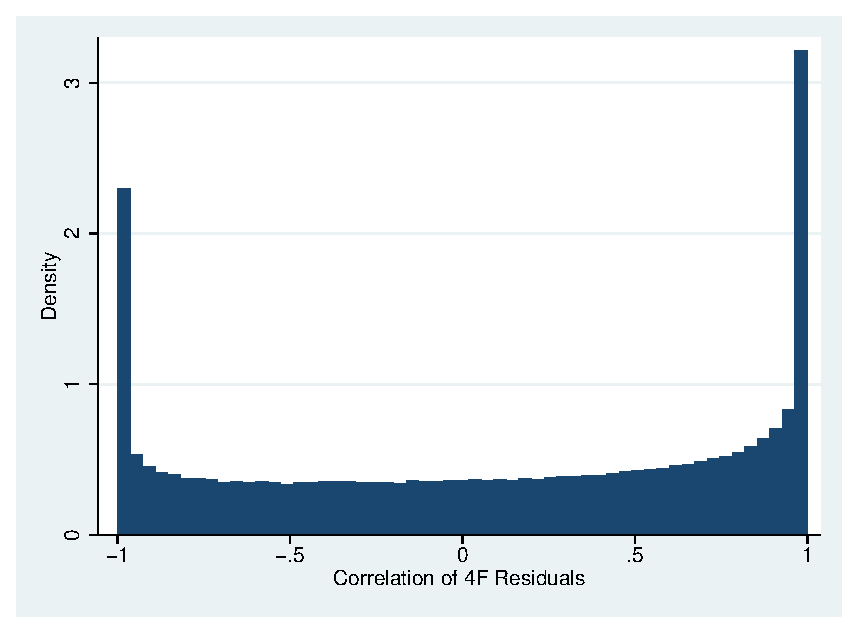
\includegraphics[width=.5\linewidth]{mygraph5.eps}\hfill
    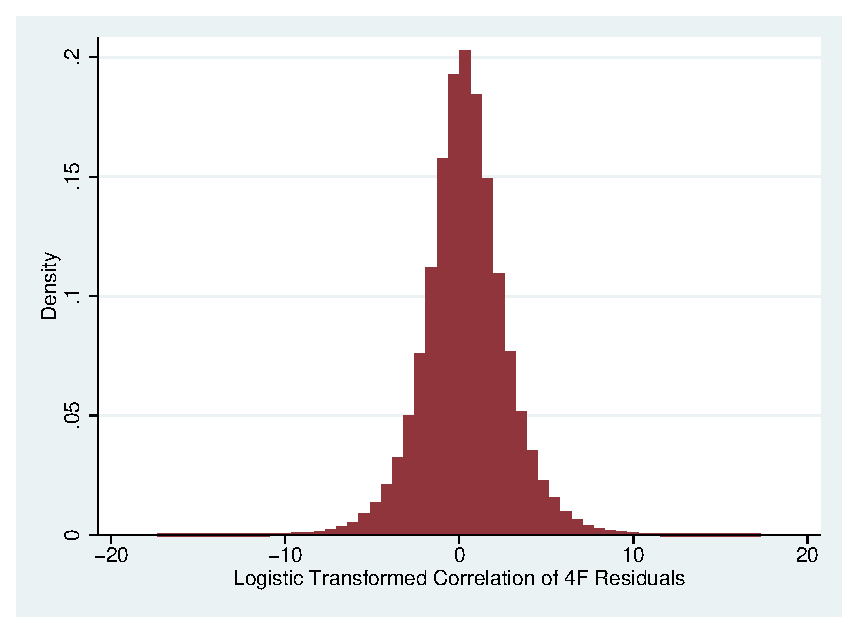
\includegraphics[width=.5\linewidth]{mygraph6.eps}\hfill
        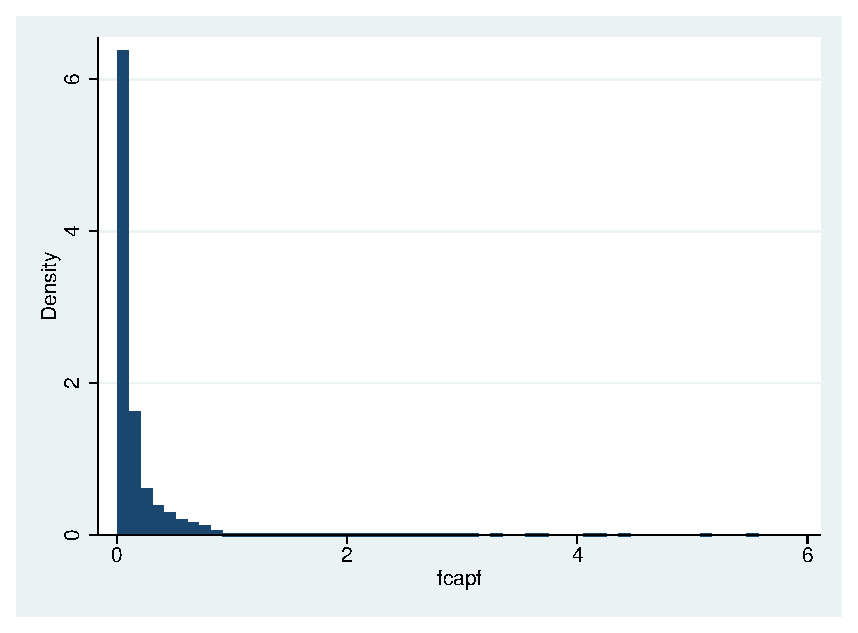
\includegraphics[width=.5\linewidth]{mygraph7.eps}\hfill
        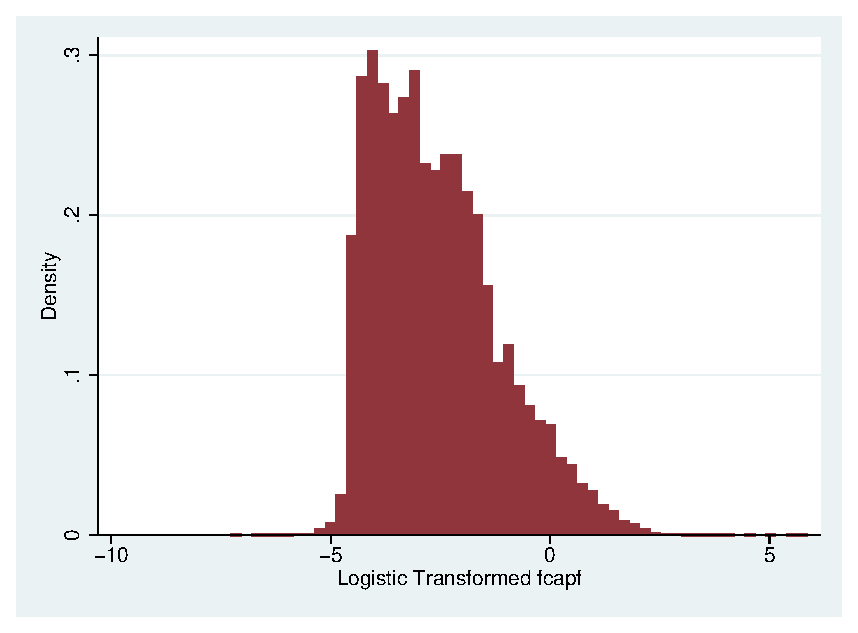
\includegraphics[width=.5\linewidth]{mygraph8.eps}
    \caption{Correlation of 4F Residuals and fcapf Logistic Transformed }
    \label{g4}
\end{figure}
\end{LTR}}





\begin{LTR}
\begin{table}
\centering
\lr{
\def\sym#1{\ifmmode^{#1}\else\(^{#1}\)\fi}
\begin{tabular}{l*{7}{c}}
\hline\hline
            &         OLS         &                     &                     &       Tobit         &                     &                     &          ML         \\
            &\multicolumn{1}{c}{(1)}&\multicolumn{1}{c}{(2)}&\multicolumn{1}{c}{(3)}&\multicolumn{1}{c}{(4)}&\multicolumn{1}{c}{(5)}&\multicolumn{1}{c}{(6)}&\multicolumn{1}{c}{(7)}\\
            &\multicolumn{1}{c}{$ l\rho4_f $}&\multicolumn{1}{c}{$ l\rho4_f $}&\multicolumn{1}{c}{$ l\rho4_f $}&\multicolumn{1}{c}{$ \rho4_f $}&\multicolumn{1}{c}{$ \rho4_f $}&\multicolumn{1}{c}{$ l\rho4_f $}&\multicolumn{1}{c}{$ l\rho4_f $}\\
\hline
            fcapf       &                     &       0.123\sym{***}&                     &      0.0351\sym{***}&      0.0382\sym{***}&       0.123\sym{***}&       0.200\sym{***}\\
                        &                     &      (4.50)         &                     &      (4.97)         &      (5.16)         &      (4.50)         &      (7.25)         \\
            [1em]
            lfcapf      &                     &                     &      0.0181\sym{***}&                     &                     &                     &                     \\
                        &                     &                     &      (5.29)         &                     &                     &                     &                     \\
[1em]
FCAPF       &      0.0287\sym{***}&                     &                     &                     &                     &                     &                     \\
            &      (5.88)         &                     &                     &                     &                     &                     &                     \\
[1em]
sgroup      &       0.482\sym{***}&       0.482\sym{***}&       0.520\sym{***}&       0.136\sym{***}&       0.136\sym{***}&       0.482\sym{***}&       0.469\sym{***}\\
            &     (33.26)         &     (32.63)         &     (35.39)         &     (35.78)         &     (34.11)         &     (32.63)         &     (31.71)         \\
[1em]
samesize    &       0.338\sym{***}&       0.346\sym{***}&       0.328\sym{***}&      0.0833\sym{***}&      0.0881\sym{***}&       0.346\sym{***}&       0.277\sym{***}\\
            &     (15.97)         &     (16.43)         &     (15.50)         &     (15.39)         &     (15.53)         &     (16.43)         &     (13.15)         \\
[1em]
$ \rho4 $         &                     &                     &                     &      0.0660\sym{***}&                     &                     &       0.249\sym{***}\\
            &                     &                     &                     &     (37.14)         &                     &                     &     (35.69)         \\
    [1em]
$ l\rho4 $         &      0.0748\sym{***}&      0.0748\sym{***}&      0.0732\sym{***}&                     &      0.0176\sym{***}&      0.0748\sym{***}&                     \\
            &     (37.53)         &     (37.56)         &     (36.71)         &                     &     (33.19)         &     (37.56)         &                     \\            
[1em]
\_cons      &       0.348\sym{***}&       0.335\sym{***}&       0.390\sym{***}&      0.0911\sym{***}&      0.0885\sym{***}&       0.335\sym{***}&       0.293\sym{***}\\
            &     (42.57)         &     (37.57)         &     (33.06)         &     (39.97)         &     (36.95)         &     (37.57)         &     (32.96)         \\
\hline
\(N\)       &      257080         &      257080         &      256920         &      311086         &      279713         &      257080         &      283716         \\
\hline\hline
\multicolumn{8}{l}{\footnotesize \textit{t} statistics in parentheses}\\
\multicolumn{8}{l}{\footnotesize \sym{*} \(p<0.05\), \sym{**} \(p<0.01\), \sym{***} \(p<0.001\)}\\
\end{tabular}
}

\caption{Other Regressions }
\label{t5}
\end{table}
\end{LTR}


\end{document}